\chapter{Electricity}

\section*{LEARNING OUTCOMES}
{
\begin{center}
\fcolorbox{black}{shadecolor}
{%
    \parbox{0.95\textwidth}
    {%
        \small
        {
           \begin{itemize}
                \item What is electricity? What is current?
                \item What are main components of an electric circuit?
                \item Current needs a closed path to flow through.
                \item What are conductors and insulators?
            \end{itemize}
        }
    }%
}
\end{center}
}

\section*{DEMONSTRATIONS}
\section*{Completion of Circuits}
To build the demonstration, you will need:

\begin{table}[H]
    \centering
    \begin{tabular}{|c|l|c|}\hline
    \textbf{\#} & \textbf{Components}  &  \textbf{Amount}\\\hline
    1   &   LED                     &   1\\\hline
    2   &   470 $\Omega$ resistors  &   1\\\hline
    3   &   Push button             &   1\\\hline
    4   &   Breadboard              &   1\\\hline
    5   &   Arduino UNO/5 V battery &   1\\\hline
    6   &   Connecting wires        &   -\\\hline
    \end{tabular}
\end{table}

\subsection*{Connections}
 Connect the push button, resistor and LED in series on the breadboard.

Fig. \ref{fig:elec-oc} illustrates the circuit.

\begin{figure}[!ht]
    \centering
    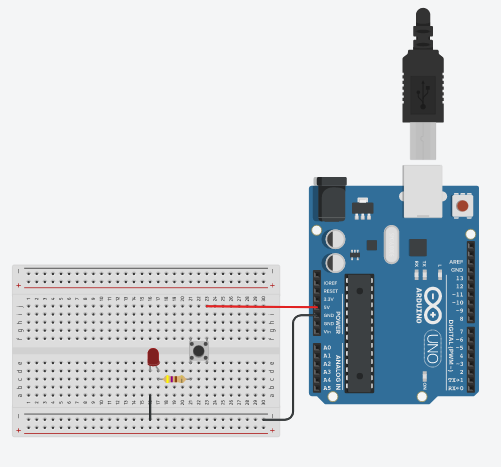
\includegraphics[scale=0.6]{Figures/electricity-open-close.PNG}
    \caption{Circuit diagram for demonstrating the completion of circuit}
    \label{fig:elec-oc}
\end{figure}

\subsection*{Procedure}
\begin{enumerate}[leftmargin=*]
    \item Press the push button and observe the state of the LED.
    \item Break the circuit from anywhere and repeat the experiment. Notice the change in the LED state.
\end{enumerate}


\subsection*{Notes}
This experiment can be modified by breaking the circuit at any place and completing it with conductors and insulators to demonstrate the flow of electricity through them.
%---------------------------------------------------------------------

\section*{2. Flow of current through series circuit}
To build the demonstration, you will need:

\begin{table}[!ht]
    \centering
    \begin{tabular}{|c|l|c|}\hline
    \textbf{\#} & \textbf{Components}  &  \textbf{Amount}\\\hline
    1   &   LED                     &   2\\\hline
    2   &   330 $\Omega$ resistor   &   1\\\hline
    3   &   Breadboard              &   1\\\hline
    4   &   Arduino UNO/5 V battery &   1\\\hline
    5   &   Connecting wires        &   -\\\hline
    \end{tabular}
\end{table}


\begin{figure}[!ht]
    \centering
    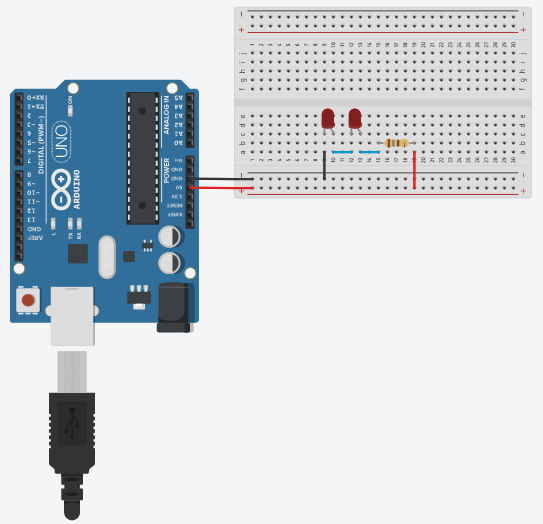
\includegraphics[scale=0.5]{Figures/electricity-series.PNG}
    \caption{Circuit diagram of series circuit}
    \label{fig:elec-s}
\end{figure}

\subsection*{Connections}
Connect two LEDs, connecting wires and resistor in series. Power the circuit either via Arduino or a 5V battery.

Fig. \ref{fig:elec-s} illustrates the aforementioned steps.

\subsection*{Procedure}
\begin{enumerate}[leftmargin=*]
    \item Observe the states of the LEDs.
    \item Break the circuit from any place and observe the state of the LEDs.
\end{enumerate}

%---------------------------------------------------------------------
\section*{3. Flow of current through parallel circuit}
To build the demonstration, you will need:

\begin{table}[!ht]
    \centering
    \begin{tabular}{|c|l|c|}\hline
    \textbf{\#} & \textbf{Components}  &  \textbf{Amount}\\\hline
    1   &   LED                     &  2\\\hline
    2   &   470 $\Omega$ resistors  &  1\\\hline
    3   &   Breadboard              &  1\\\hline
    4   &   Arduino UNO/5 V battery &  1\\\hline
    5   &   Connecting wires        &  -\\\hline
    \end{tabular}
\end{table}

\subsection*{Connections}
\begin{enumerate}[leftmargin=*]
    \item Connect the LEDs in parallel. 
    \item Connect the resistor in series with LED and connect it to the parallel combination of LEDs.
    \item Power the circuit via Arduino or a 5V battery.
\end{enumerate}
Fig. \ref{fig:elec-p} illustrates the aforementioned steps.

\subsection*{Procedure}
\begin{enumerate}[leftmargin=*]
    \item Observe the states of the LEDs.
    \item Remove any LED and observe the state of the other LED.
    \item Place the LED back in the circuit and repeat the previous step with the other LED.
\end{enumerate}
\begin{figure}[H]
    \centering
    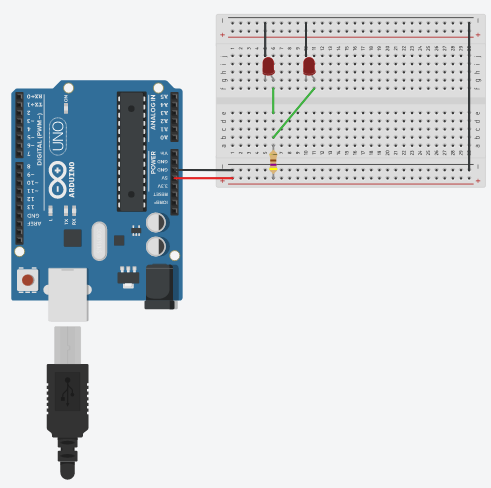
\includegraphics[scale=0.6]{Figures/electricity-parallel.PNG}
    \caption{Circuit diagram of parallel circuit}
    \label{fig:elec-p}
\end{figure}
\vfill